\subsection{Протоколы транспортного уровня в промышленных сетях}
Протоколы транспортного уровня предназначены для доставки данных. При этом неважно, какие данные передаются, откуда и куда, протокол предоставляет сам механизм передачи. Блоки данных он разделяет на фрагменты, размеры которых зависят от протокола: короткие объединяет в один, а длинные разбивает. Протоколы этого уровня предназначены для взаимодействия типа точка-точка. 

На \refris{fig:osi} показана структура идеальной модели \textit{OSI}. Модель определяет различные уровни взаимодействия систем. Каждый уровень выполняет определённые функции при таком взаимодействии.

\begin{figure}[H]
	\centering
	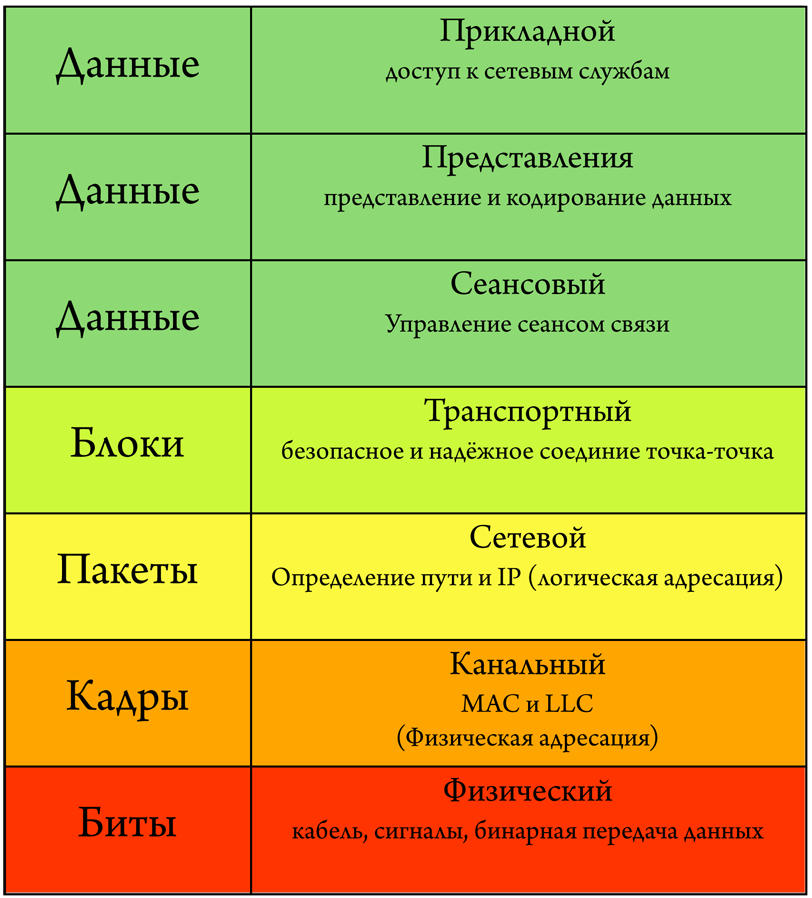
\includegraphics[width=0.4\linewidth]{images/osi}
	\caption{Уровни модели OSI}
	\label{fig:osi}
\end{figure}

В настоящее время двумя самыми популярными протоколами являются \textit{TCP} и \textit{UDP}.
\subsubsection{Уровни модели OSI}
Из \refris{fig:osi} и \cite{kumar_survey_2012} уровни модели OSI делятся на:
\begin{itemize}
	\item \textbf{физический}: предназначен непосредственно для передачи потока данных. Осуществляет передачу электрических или оптических сигналов в кабель или в радиоэфир и, соответственно, их приём и преобразование в биты данных в соответствии с методами кодирования цифровых сигналов;
	\item \textbf{канальный}: полученные с физического уровня данные проверяет на ошибки, если нужно исправляет, упаковывает во фреймы, проверяет на целостность, и отправляет на сетевой уровень;
	\item \textbf{сетевой}: определяет пути передачи данных. Отвечает за трансляцию логических адресов и имён в физические, за определение кратчайших маршрутов, коммутацию и маршрутизацию, за отслеживание неполадок и заторов в сети;
	\item \textbf{транспортный}: организует доставку данных без ошибок, потерь и дублирования (не все) в той последовательности, как они были переданы. Разделяет данные на фрагменты равной величины, объединяя короткие и разбивая длинные (размер фрагмента зависит от используемого протокола);
	\item \textbf{сеансовый}: управляет созданием/завершением сеанса связи, обменом информацией, синхронизацией задач, определением права на передачу данных и поддержанием сеанса в периоды неактивности приложений. Синхронизация передачи обеспечивается помещением в поток данных контрольных точек, начиная с которых возобновляется процесс при нарушении взаимодействия;
	\item \textbf{представления}: на этом уровне может осуществляться преобразование протоколов и сжатие/распаковка или кодирование/декодирование данных, а также перенаправление запросов другому сетевому ресурсу, если они не могут быть обработаны локально;
	\item \textbf{прикладной}: уровень приложений (англ. Application layer). Обеспечивает взаимодействие сети и приложений пользователя, выходящих за рамки модели OSI. На этом уровне работают изученные в работе протоколы автоматизации промышленных сетей.
\end{itemize}
\subsubsection{Транспортный протокол TCP}
\textbf{TCP} \cite{noergaard_chapter_2010} -- один из основных протоколов транспортного уровня. Он обеспечивает надёжную доставку потока байтов от одного устройства к другому. \textit{TCP} ориентирован на качество соединения, а не на скорость. В нём присутствует механизм признания (acknowledgement) и механизм предотвращения скоплений, что уменьшает передачу в то время, как сеть загружена. 

Этот протокол можно назвать стабильным, поскольку он способен адаптироваться к различным ситуациям, происходящим в сети. После отправки пакета в сеть, он сохраняется в буфере и дожидается пакета, подтверждающего получение данных приёмником, что крайне важно при передаче данных с приборов. 

\paragraph{Функции TCP}
\begin{itemize}
	\item \textbf{передача данных}: передаёт непрерывный поток данных в форме сегментов для передачи через сеть;
	\item \textbf{надёжная доставка}: пакеты ACK (см. \refpar{par:tcpstruct}) помогают удостовериться в том, что пакет получен там, где необходимо;
	\item \textbf{управление потоком}: получатель контролирует объём полученных данных при помощи возврата ``окна'' с каждым пакетом ACK. В этом окне содержится то количество данных, которое готов принять приёмник;
	\item \textbf{мультиплексирование}: возможность использовать несколько портов для одновременного обмена данными. Объединение адреса сети и хоста образует \gls{socket}.
\end{itemize}
\paragraph{Структура TCP пакета}\label{par:tcpstruct}
На \refris{fig:pole-tcp} приведена структура TCP.
\begin{figure}[h]
	\centering
	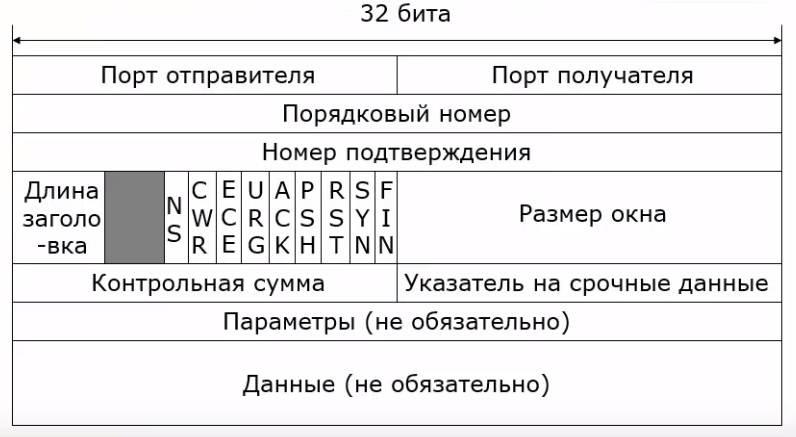
\includegraphics[width=0.8\linewidth]{images/pole-tcp}
	\caption{Структура TCP сегмента}
	\label{fig:pole-tcp}
\end{figure}
Краткое резюме по полям:
\begin{itemize}
	\item \textbf{порт отправителя}: 16-ти битный номер, определяющий отправителя пакета;
	\item \textbf{порт получателя}: 16-ти битный номер, который отправитель использует для отправки пакета получателю;
	\item \textbf{порядковый номер}: в этом поле содержится первый номер байта в сегменте;
	\item \textbf{номер подтверждения (ACK)}: обеспечивает гарантию доставки сообщений. Например, был получен байт $2459$, значит в пакете ACK будет передан следующий ожидаемый байт -- $2460$;
	\item \textbf{длина заголовка}: число 32-х разрядных слов в заголовке;
	\item \textbf{резерв}: 3 - 6 битов, зарезервированные для дальнейшего развития протокола и установлены на значение 0;
	\item \textbf{контрольные биты (флаги)}: определяют использование сегмента или служат проверкой действительности для других полей:
	\begin{itemize}
		\item \textbf{NS}: экспериментальный флаг, используется для защиты от случайного злонамеренного сокрытия пакетов от отправителя;
		\item \textbf{CWR}: используется хостом, чтобы указать, что он получил пакет с установленным флагом \textit{ECE};
		\item \textbf{ECE}: получатель поддерживает ECN (взаимное уведомление хоста и пира о переполнении канала без потери пакетов);
		\item \textbf{URG}: флаг срочности используется для уведомления получателя о необходимости обработки срочных пакетов перед обработкой всех других пакетов. Получатель будет уведомлен, когда будут получены все известные срочные данные. В \reftab{tab:psh-urg} приводится отличие флагов \textit{PSH} и \textit{URG};;
		\item \textbf{ACK}: используется для подтверждения успешного получения пакета;
		\item \textbf{PSH}: используется для информирования отправителя о том, что требуется более высокая пропускная способность, поэтому, если возможно, данные должны передаваться с более высокой пропускной способностью, то есть отправленных пакетов будет больше, однако скорость обмена информацией будет быстрее (что критично для систем реального времени). В \reftab{tab:psh-urg} приводится отличие флагов \textit{PSH} и \textit{URG};
		\begin{table}[b]
			\centering
			\caption{Отличие флагов PSH и URG}
			\label{tab:psh-urg}
			\begin{tabular}{|C{0.4\linewidth}|C{0.4\linewidth}|}
				\hline
				\bfseries PSH & \bfseries URG\\
				\hline
				Все данные из буфера передаются отправителю/приёмнику&Только данные, помеченные флагом \textit{URG} будут переданы приёмнику (немедленно)\\
				\hline
				Данные отправляются последовательно & Данные передаются в случайном порядке\\
				\hline
			\end{tabular}
		\end{table}
		
		\item \textbf{RST}: используется для сброса TCP-соединения при возникновении путаницы в порядковых номерах. В \reftab{tab:fin-rst} приведено отличие \textit{FIN} от \textit{RST};
		\item \textbf{SYN}: флаг синхронизации используется в качестве первого шага в установлении трехстороннего рукопожатия между двумя хостами. Этот флаг должен быть установлен только для первого пакета от отправителя и получателя. На \refris{fig:handshake} показан процесс трехстороннего рукопожатия; 
		\begin{figure}[t]
			\centering
			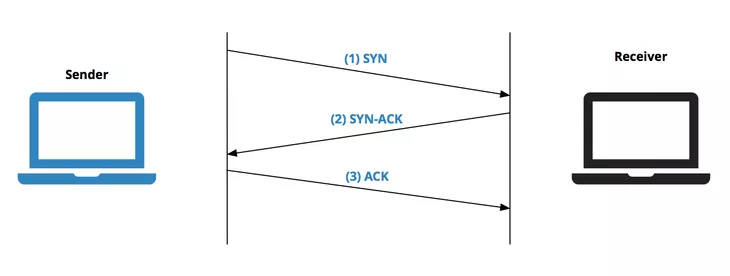
\includegraphics[width=0.8\linewidth]{images/handshake}
			\caption{Трёхстороннее рукопожатие с пакетом SYN}
			\label{fig:handshake}
		\end{figure}
		\item \textbf{FIN}: флаг завершения означает, что от отправителя больше нет данных. Следовательно, он используется в последнем пакете, отправленном отправителем. В \reftab{tab:fin-rst} приведено отличие \textit{FIN} от \textit{RST};
		
		\begin{table}[h]
			\centering
			\caption{Отличие флагов PSH и URG}
			\label{tab:fin-rst}
			\begin{tabular}{|C{0.4\linewidth}|C{0.4\linewidth}|}
				\hline
				\bfseries FIN & \bfseries RST\\
				\hline
				Аккуратно завершает соединение&Резко сообщает другой стороне общения о завершении передачи\\
				\hline
				Нет потери данных & Данные сбрасываются\\
				\hline
				Устройство, получившее этот флаг может продолжать делать запросы & Получатель этого флага должен перестать передавать данные\\
				\hline
			\end{tabular}
		\end{table}
	\end{itemize}
	
	\item \textbf{размер окна}:  в этом поле получатель указывает, сколько данных он может принять. Поле используется для управления потоком;
	\item \textbf{контрольная сумма}: используется для проверки правильности доставки данных, если контрольная сумма, рассчитанная получателем, не совпадает с контрольной суммой в заголовке TCP, то этот сегмент отбрасывается;
	\item \textbf{указатель на срочные данные}: поле указывает порядковый номер октета, которым заканчиваются важные (urgent) данные. Поле принимается во внимание только для пакетов с установленным флагом URG;
	\item \textbf{параметры}: необязательный параметр, применяемый для тестирования и увеличения пропускной способности канала;
	\item \textbf{данные}: сообщение протокола верхнего уровня.
\end{itemize}

\paragraph{Применение TCP}
Технология TCP применяется в следующих областях \cite{kumar_survey_2012}:
\begin{enumerate}
	\item \textbf{HTTP}: самый распространённый протокол передачи данных по сети;
	\item \textbf{FTP}: протокол обмена данными по сети; 
	\item \textbf{IMAP}: доступ к электронной почте;
	\item \textbf{POP}: доступ к электронной почте;
	\item \textbf{RLogin}: удалённый доступ к оборудованию;
	\item \textbf{SMTP}: доступ к электронной почте;
	\item \textbf{SSH}: создание защищённых соединений для удалённого доступа;
	\item \textbf{Modbus TCP}: протокол Modbus, ``завёрнутый'' в оболочку TCP.
\end{enumerate}

\subsubsection{Протокол UDP}
\textbf{UDP} \cite{kumar_survey_2012} -- один из основных протоколов обмена данными. Хост отправляет сообщения в форме датаграммы без предварительной установки соединения. Подходит для случаев, когда важна скорость, а не гарантия доставки. 

\paragraph{Структура UDP датаграммы}
На \refris{fig:udp} приведена структура UDP датаграммы.
\begin{figure}[h]
	\centering
	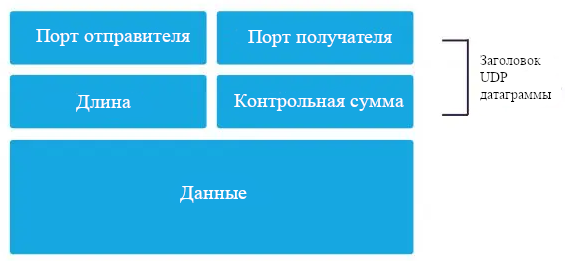
\includegraphics[width=0.8\linewidth]{images/udp}
	\caption{Структура UDP датаграммы}
	\label{fig:udp}
\end{figure}
Краткое резюме по всем полям:
\begin{itemize}
	\item \textbf{source port (порт отправителя)}: порт процесса, который отправляет датаграмму;
	\item \textbf{destination port (порт назначения)}: порт процесса, принимающего датаграмму;
	\item \textbf{length (длина)}: длина датаграммы (вместе с \textit{Header});
	\item \textbf{checksum (контрольная сумма)}: опциональное поле. Контрольная сумма позволяет принимающему устройству проверять целостность заголовка пакета и полезной нагрузки. Это необязательно в IPv4, но стало обязательным в IPv6;
	\item \textbf{data (данные)}: передаваемые пакетом данные.
\end{itemize}
\subsubsection{Сравнение TCP и UDP}
По теоретическим данным \cite{kumar_survey_2012, noergaard_chapter_2010} и экспериментальным данным \cite{hussein_wheeb_performance_2015}, можно сделать следующие выводы: 

\begin{longtable}{|C{8cm}|C{8cm}|}
	\caption{Сравнительная таблица TCP и UDP}
	\label{tab:tcp_udp}\\
	\hline
	\bfseries TCP & \bfseries UDP\\
	\endfirsthead
	\hline
	TCP & UDP\\
	\endhead
	\hline
	Надёжное соединение без перегрузки сети & Не гарантирует надёжность и порядок отправляемых пакетов\\
	\hline
	Создание подключения осуществляется при помощи 3 рукопожатий, см \refris{fig:handshake}. После установки соединения данные передаются в обе стороны \cite{kumar_survey_2012} & Сразу отправляет данные \cite{noergaard_chapter_2010}\\
	\hline
	Пропускная способность \cite{hussein_wheeb_performance_2015} (количество успешно принятых пакетов) у TCP составила $740$ kbps & Пропускная способность \cite{hussein_wheeb_performance_2015} у UDP составила $586$ kbps\\
	\hline
	Задержка у TCP составила $0.059$ ms \cite{hussein_wheeb_performance_2015} & Задержка у UDP составила $0.051$ ms \cite{hussein_wheeb_performance_2015}\\
	\hline
	TCP потерял $8$ пакетов \cite{hussein_wheeb_performance_2015} & UDP потерял $311$ пакетов \cite{hussein_wheeb_performance_2015}\\
	\hline
	TCP доставил $96.92\%$ пакетов \cite{hussein_wheeb_performance_2015} & UDP доставил $74.12\%$ пакетов \cite{hussein_wheeb_performance_2015}\\
	\hline
	TCP применяется там, где необходима надёжность соединения & UDP примняется там, где время играет ключевую роль\\
	\hline
\end{longtable}

\subsubsection{Вывод}
После рассмотрения протоколов транспортного уровня, можно сделать вывод, что для автоматизации вакуумной установки лучше всего пойдёт \textit{TCP}, поскольку в нашем случае важнее не скорость отправки и получения, а надёжность соединения.

Хочется отметить, что хоть TCP и медленнее, но он теряет гораздо меньше пакетов, доставляет куда больший процент пакетов и экономит трафик, поскольку нет необходимости в повторной отравке потерянных пакетов \cite{kumar_survey_2012}. 

Как показала практика, задержки у TCP не сильно выше, чем у UDP \cite{hussein_wheeb_performance_2015}.